\documentclass[aspectratio=169]{beamer}

\usepackage[utf8]{inputenc}
\usepackage[TS1,T1]{fontenc}
\usepackage{amsmath}
\usepackage{biblatex}
\usepackage{graphicx}
\usepackage{ctex}
\usepackage{framed}
\usepackage{quiver}
\usepackage{tikz-cd}
\usepackage{float}

\setlength{\FrameRule}{0.5pt} % 设置边框线的宽度
\setlength{\FrameSep}{10pt} % 设置边框线与内容之间的间距
\setlength{\leftmargin}{0pt} % 将左边框与左边距对齐

\usepackage{tikz}
\usetikzlibrary{decorations.pathreplacing}
\usetikzlibrary{positioning}

\newcommand{\tikzmark}[3][]
  {\tikz[remember picture, baseline]
    \node [anchor=base,#1](#2) {#3};}

\addbibresource{references.bib} % Specify the bibliography file

\title{\Large{\bfseries{不定方程相关理论及其应用}}}
\date{\scriptsize{\today}}
\author{\small{\fangsong{郑欢誉}}}

\usetheme[language=english]{LTU}

\begin{document}
	
	\begin{frame}
		\titlepage
	\end{frame}
    
   	\begin{frame}{中期报告目录}{\small{Contents of Interim Report}}
       \liwicki[1]{研究内容和目标\small{Research Contents \& Object}}\\
       \liwicki[2]{当前进展\small{Current Progress}}\\
       \liwicki[3]{未来计划\small{Future Plan}}\\
   	\end{frame}
	
	\begin{frame}{研究内容和目标}{Research Contents \& Object}
        \begin{framed}
		$$
        x^n + y^n = z^n
        $$
        \begin{center}
            当$n \geq 3$为\underline{正规素数}时,方程没有非零整数解$(x, y, z)$
        \end{center}
        \end{framed}
        \begin{enumerate}
        \item FLT \& ABC猜想(ABC $\Longrightarrow$ FLT,ABC猜想次指数界改良)
        \item 渐进费马大定理(Asymptotic Fermat's Last Theorem)
        \item 正规素数情况的形式化
        \end{enumerate}
	\end{frame}
	
	\begin{frame}{当前进展}{Current Progress}
        \begin{figure}[htpb]
        \centering
        \begin{minipage}{0.49\linewidth}
        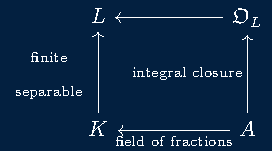
\includegraphics[width=6.2cm]{dia1.pdf}
        \end{minipage}
        \begin{minipage}{0.49\linewidth}
        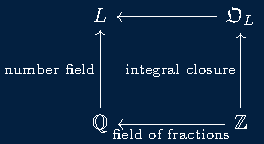
\includegraphics[width=6.2cm]{dia2.pdf}
        \end{minipage}
        \end{figure}
	\end{frame}
    
	\begin{frame}{当前进展}{Current Progress}
        \begin{figure}[htpb]
        \centering
        \begin{minipage}{0.49\linewidth}
        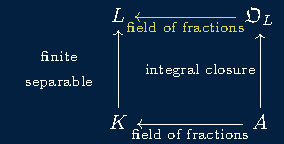
\includegraphics[width=6.2cm]{dia3.pdf}
        \end{minipage}
        \hfill
        \begin{minipage}{0.49\linewidth}
        $\mathfrak{O}_L$:
        \begin{enumerate}
        \item \textcolor{rgb,255:red,214;green,214;blue,92}{forms a ring}
        \item (when $A$ is PID) finitely generated $A$-module
        \end{enumerate}
        \end{minipage}
        \end{figure}
	\end{frame}
    
   	\begin{frame}{当前进展}{Current Progress}
        \begin{figure}[htpb]
        \centering
        \begin{minipage}{0.49\linewidth}
        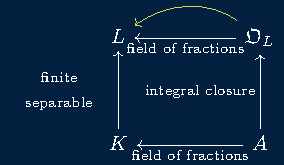
\includegraphics[width=6.2cm]{dia4.pdf}
        \end{minipage}
        \hfill
        \begin{minipage}{0.49\linewidth}
        $\mathfrak{O}_L$:
        \begin{enumerate}
        \item forms a ring
        \item (when $A$ is PID) \tikzmark{a0}{\textcolor{rgb,255:red,214;green,214;blue,92}{finitely generated $A$-module}}
        \begin{tikzpicture}[overlay, remember picture]
            \node[white] (a0d) [left=of a0, xshift=-0.6cm, yshift=3cm]{\textcolor{rgb,255:red,214;green,214;blue,92}{integral basis is a $K$-basis for $L$}};
            \draw[white,->,] (a0.east) to [in=0,out=90] (a0d.east);
        \end{tikzpicture}
        \end{enumerate}
        \end{minipage}
        \end{figure}
   	\end{frame}

    \begin{frame}{当前进展}{Current Progress}
        \begin{figure}[htpb]
        \centering
        \begin{minipage}{0.49\linewidth}
        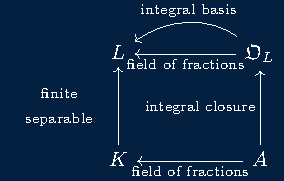
\includegraphics[width=6.2cm]{dia5.pdf}
        \end{minipage}
        \hfill
        \begin{minipage}{0.49\linewidth}
        $\mathfrak{O}_L$:
        \begin{enumerate}
        \item forms a ring
        \item (when $A$ is PID) finitely generated $A$-module
        \item \textcolor{rgb,255:red,214;green,214;blue,92}{Noetherian ($\Rightarrow$ factorization of ideal into irreducibles)}
        \end{enumerate}
        \end{minipage}
        \end{figure}
    \end{frame}
    
    \begin{frame}{当前进展}{Current Progress}
        \begin{figure}[htpb]
        \centering
        \begin{minipage}{0.49\linewidth}
        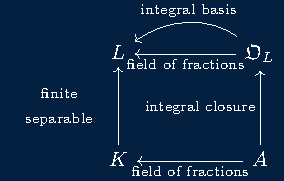
\includegraphics[width=6.2cm]{dia5.pdf}
        \end{minipage}
        \hfill
        \begin{minipage}{0.49\linewidth}
        $\mathfrak{O}_L$:
        \begin{enumerate}
        \item forms a ring
        \item (when $A$ is PID) finitely generated $A$-module
        \item Noetherian ($\Rightarrow$ factorization of ideal into irreducibles)
        \item \textcolor{rgb,255:red,214;green,214;blue,92}{Dedekind 
        \\ ($\Rightarrow$ fractional ideal, inverse of ideal)
        \\ ($\Rightarrow$ unique prime factorization of ideal)}
        \end{enumerate}
        \end{minipage}
        \end{figure}
    \end{frame}
    
    \begin{frame}{当前进展}{Current Progress}
        \begin{figure}[htpb]
        \centering
        \begin{minipage}{0.49\linewidth}
            $\mathfrak{O}_L$:
            \begin{enumerate}
            \item forms a ring
            \item (when $A$ is PID) finitely generated $A$-module
            \item Noetherian ($\Rightarrow$ factorization of ideal into irreducibles)
            \item \textcolor{rgb,255:red,214;green,214;blue,92}{Dedekind 
            \\ ($\Rightarrow$ fractional ideal, inverse of ideal)
            \\ ($\Rightarrow$ unique prime factorization of ideal)}
            \end{enumerate}
        \end{minipage}
        \hfill
        \begin{minipage}{0.49\linewidth}
        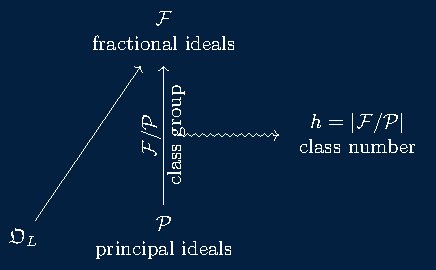
\includegraphics{dia6.pdf}
        \end{minipage}
        \end{figure}
    \end{frame}
    
    \begin{frame}{当前进展}{Current Progress}
        \begin{figure}[htpb]
        \centering
        \begin{minipage}{0.49\linewidth}
        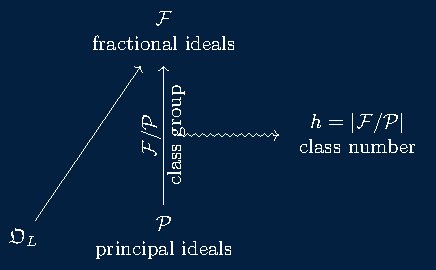
\includegraphics{dia6.pdf}
        \end{minipage}
        \hfill
        \begin{minipage}{0.49\linewidth}
        Minkowski's Theorem
        \begin{flalign}
        \notag
        \Rightarrow& \text{class number finite} \\
        \notag
        \Rightarrow& \textcolor{rgb,255:red,214;green,214;blue,92}{q\text{ coprime to }h, \ \mathfrak{a}^q \text{ principal,}} \\ 
        \notag
        &\textcolor{rgb,255:red,214;green,214;blue,92}{\text{then }\mathfrak{a}\text{ principal}}
        \end{flalign}
        \end{minipage}
        \end{figure}
    \end{frame}
    
    \begin{frame}{当前进展}{Current Progress}
    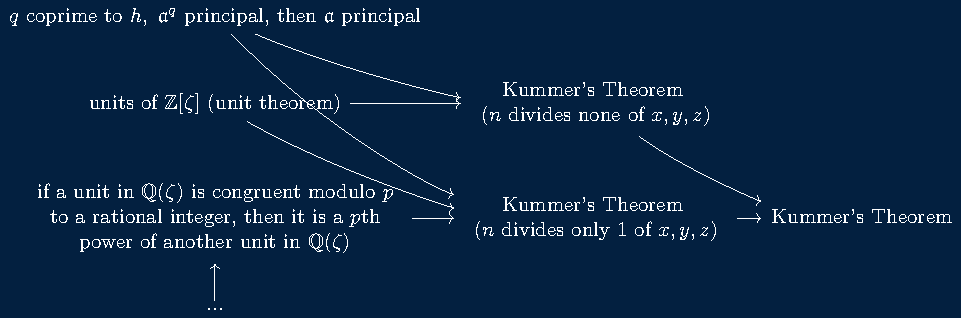
\includegraphics[width=\linewidth]{dia7.pdf}
    \end{frame}
    
    \begin{frame}{当前进展}{Current Progress}
        \begin{figure}[htpb]
        \centering
        \begin{minipage}{0.49\linewidth}
        \centering
        
\includegraphics[width=0.6\linewidth]{screenshot1.png}
        \end{minipage}
        \hfill
        \begin{minipage}{0.49\linewidth}
        \textbf{Lean} is an \underline{interactive theorem prover} based on \underline{dependent type theory}, designed for use both in cutting-edge mathematics and in software verification.
        \end{minipage}
        \end{figure}
    \end{frame}
    
    \begin{frame}{当前进展}{Current Progress}
    \centering
    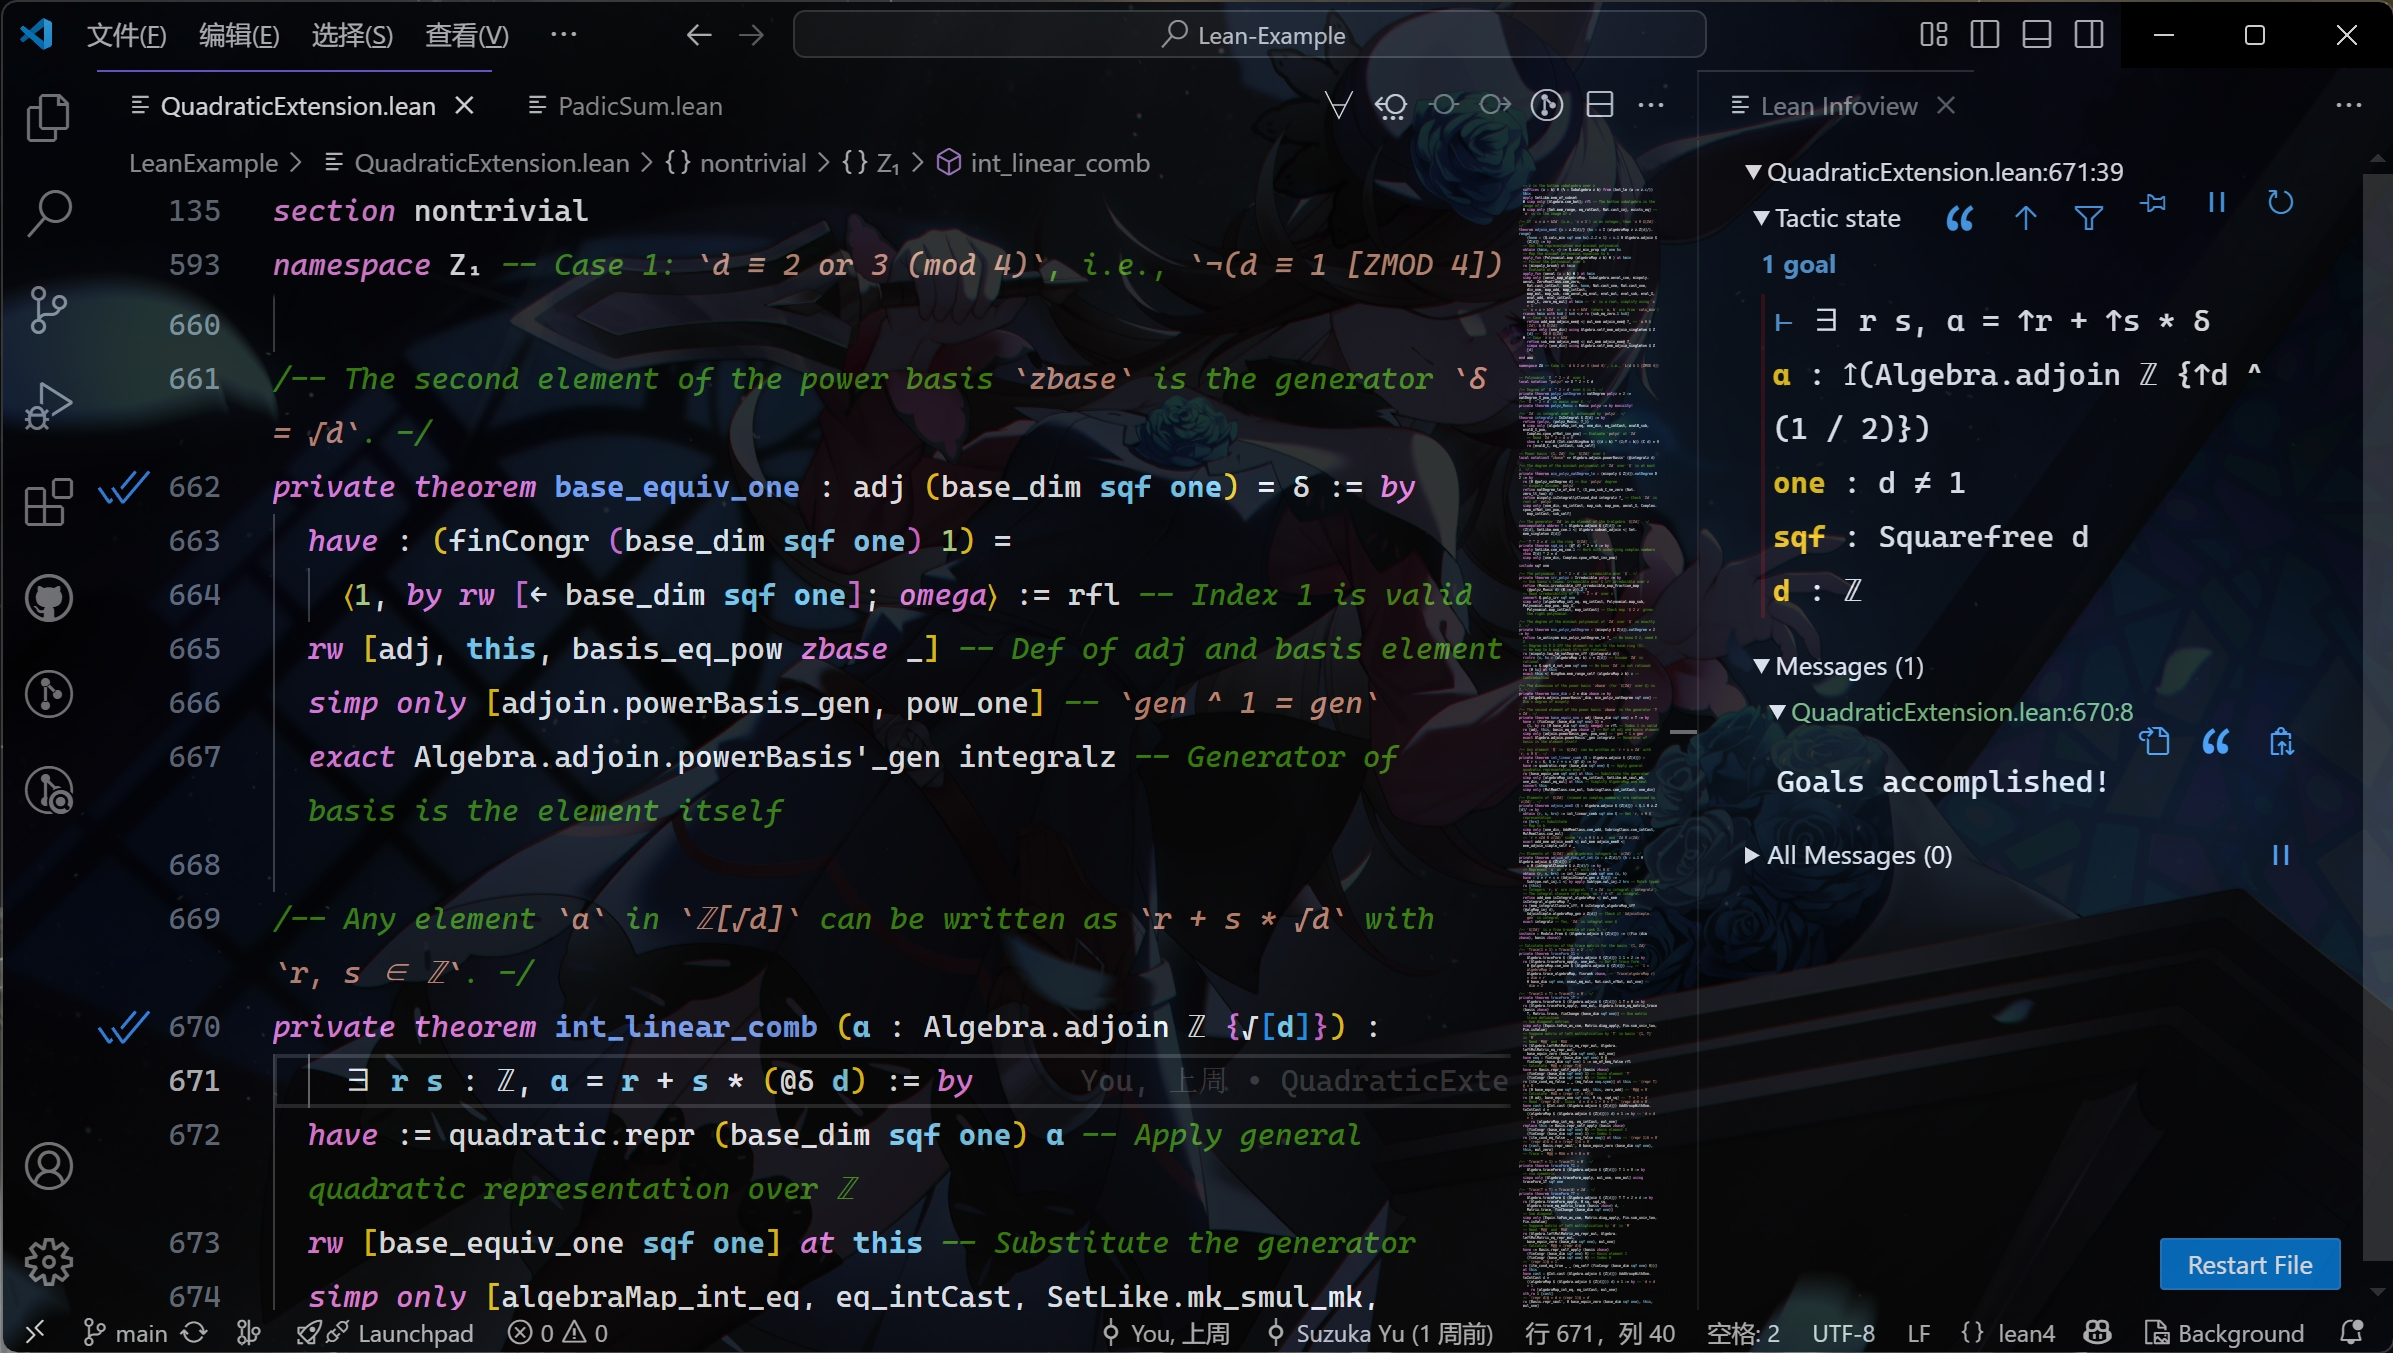
\includegraphics[width=0.8\linewidth]{screenshot2.png}
    \end{frame}
    
    \begin{frame}{当前进展}{Current Progress}
    \centering
    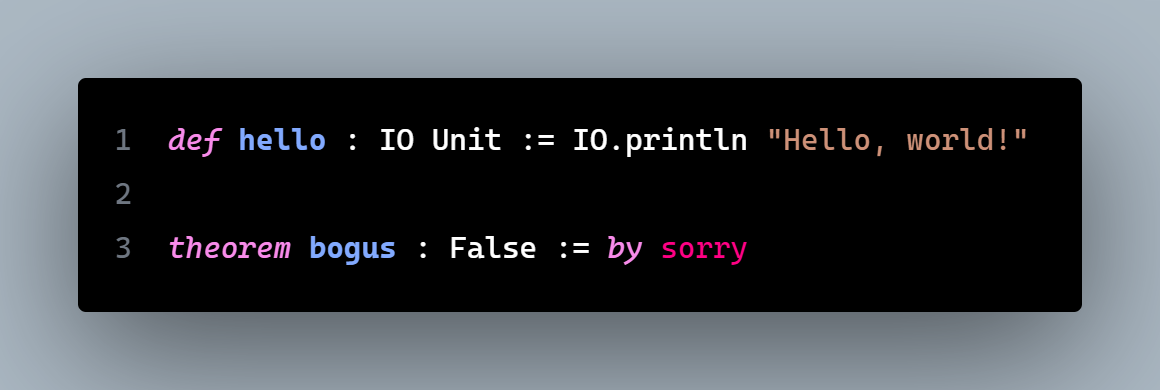
\includegraphics[width=0.8\linewidth]{screenshot3.png}
    \end{frame}
    
    \begin{frame}{当前进展}{Current Progress}
    相关实验:
    \begin{enumerate}
    \item (1300行)The discriminate of a quadratic extension $\mathbb{Q}(\sqrt{d})$, where $d$ is a square free integer is
    \[
    \left\{\begin{matrix}
    d,  & d \equiv 1 \ (mod \ 4)\\
    4d,  & d \not\equiv 1 \ (mod \ 4)
    \end{matrix}\right.
    \]
    \item (100行)Every epimorphism of Grps is the coequalizer of two homomorphisms.
    \item (200行)Every monomorphism of Grps is the equalizer of two homomorphisms.
    \item (200行)Let $0 \neq x \in \mathbb{Q}$. $|x| (\prod_{p \text { prime }}|x|_{p})=1$
    \end{enumerate}
    \end{frame}
    
    \begin{frame}{未来计划}{Future Plan}
    \begin{enumerate}
    \item FLT \& ABC猜想(ABC $\Longrightarrow$ FLT,ABC猜想次指数界改良)
    \item 渐进费马大定理(Asymptotic Fermat's Last Theorem)
    \item 正规素数情况的形式化
    \end{enumerate}
    \end{frame}
\end{document}